\section{Diseño de los programas}
\subsection{Diagrama de flujo del osciloscopio}
El osciloscopio se puede implementar en el Arduino UNO siguiendo el diagrama de flujo que se ilustra en la figura \ref{fsm}. Por un lado, en AC se debe muestrear múltiples veces para determinar el valor máximo de una señal senoidal. Luego el proceso anterior se debe repetir varias veces tal que se obtiene el último valor máximo así como valores máximos pasados. Esto permite que ante un cambio en la amplitud de la señal senoidal, en especial una disminución, el medidor puede registrar el cambio y mostrar el valor correcto en pantalla.
Por otro lado, en DC también se conserva varias lecturas anteriores además de la lectura más reciente, esto para calcular el valor promedio.
\begin{figure}[H]
    \centering
    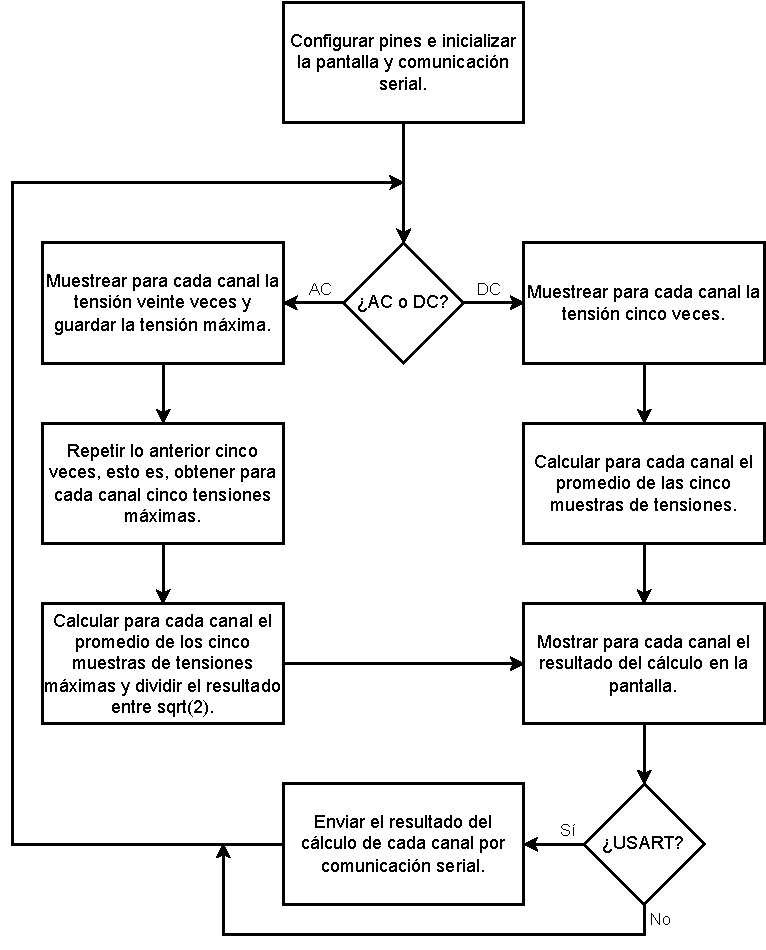
\includegraphics[width=14cm]{Imagenes/fsm.pdf}
    \caption{Diagrama de flujo del programa en el Arduino UNO.}
    \label{fsm}
\end{figure}

Ahora, en la figura \ref{fsm-py} se ilustra el diagrama de flujo del programa utilizado para recibir las lecturas por comunicación serial y guardarlo en un archivo csv. La implementación para configurar y abrir el puerto serial en Python se puede consultar en \cite{serial}.
\subsection{Diagrama de flujo del capturador de datos}
\begin{figure}[H]
    \centering
    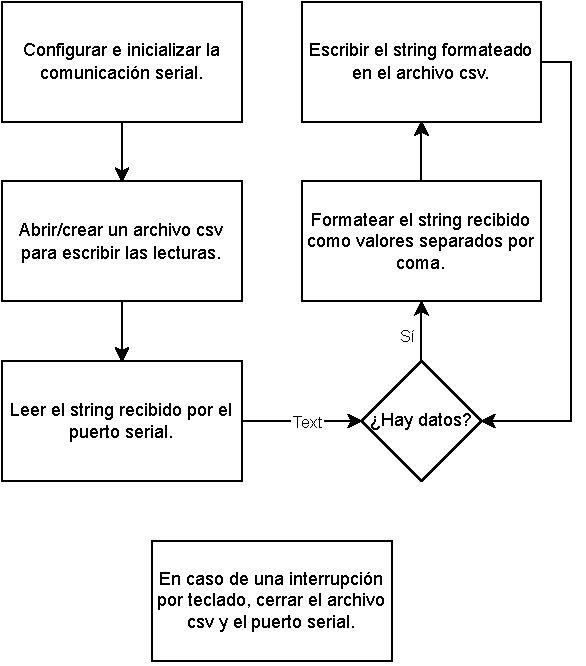
\includegraphics[width=10cm]{Imagenes/fsm_py.pdf}
    \caption{Diagrama de flujo del programa que captura y guarda las lecturas de tensiones.}
    \label{fsm-py}
\end{figure}